\section{Theorie hinter Deep Learning}

Das \ac{dl} stellt einen spezialisierten Teilbereich des \ac{ml} dar, welcher auf der Verwendung tiefer neuronaler Netzwerke basiert. Die theoretischen Grundlagen für \ac{dl} , insbesondere im Bereich neuronaler Architekturen und Lernalgorithmen, wurden von \citet[S. 22-40]{Lang:2023} umfassend behandelt. In den folgenden Unterkapiteln (3.1 bis 3.9) wird ein Großteil dieser Ausführungen aufgegriffen und systematisch erläutert. Die zugrundeliegenden Formeln stammen hauptsächlich aus \citeauthor{Lang:2023}s Werk. Eine Ausnahme bildet Unterkapitel 3.5, in dem die Formeln und Ansätze auf den Arbeiten von \citet[]{Tiwari:2022} sowie \citet[]{Grandini:2020} basieren.

\subsection{Tiefe neuronale Netze}

Der grundlegende Ansatz hinter \ac{dl}-Algorithmen basiert auf der Idee, künstliche neuronale Netzwerke zu entwickeln, die die Funktionsweise des menschlichen Gehirns nachahmen (vgl. \citealt[S. 279]{Geron:2019}). Dieses Konzept wurde von \citet[]{Rosenblatt:1958} durch das Perzeptron-Modell eingeführt, welches als probabilistisches Modell für die Informationsspeicherung und -organisation im Gehirn dient. Die Bildung von Verbindungen zwischen künstlichen Neuronen erfolgt in ähnlicher Weise wie die neuronale Kommunikation im Gehirn, nämlich durch wiederholtes Training und entsprechende Anpassung der Gewichtungen (vgl. \citealt[S. 286-287]{Geron:2019}).\\
Ein künstliches Neuron multipliziert einen Eingangsvektor \(
\mathbf{x} = (x_1, x_2, \ldots, x_n)
\) mit einem Gewichtungsvektor \(
\mathbf{w} = (w_1, w_2, \ldots, w_n)
\), um ein skalares Signal zu bilden und addiert ein Bias-Term \(b\), um ein Logit zu erzeugen, das durch eine Aktivierungsfunktion \(f\) in das Ausgabesignal 
\begin{equation}
\begin{aligned} 
y(\mathbf{x}; \mathbf{w}, b) = f(\mathbf{x} \cdot \mathbf{w} + b)
\end{aligned} 
\end{equation}
umgewandelt wird.\\
Rosenblatts Modell eines künstlichen Neurons, das Perzeptron, verwendete die Heaviside-Stufenfunktion als Aktivierungsfunktion und einen negativen Bias-Term, um eine binäre Ausgabe zu erzeugen:
\begin{equation}
\begin{aligned}
y = \begin{cases}
1 & \text{wenn} \sum_{j} x_j \cdot w_j > b \\
0 & \text{wenn} \sum_{j} x_j \cdot w_j \leq b.
\end{cases}
\end{aligned} 
\end{equation}
Die Lösung komplexer Modellierungsprobleme erfordert die Verwendung komplexer Modelle, die über die Fähigkeiten eines einzelnen Perzeptrons hinausgehen. Eine Möglichkeit der Modellierung ist die Kombination mehrerer Perzeptrons zu einem Netzwerk, welches als \ac{mlp} bezeichnet wird. Layer, welche nicht direkt mit der Eingabe oder Ausgabe verbunden sind, werden als versteckte Schichten (engl. \textit{hidden layer}) bezeichnet. Modelle, die zwei oder mehr versteckte Schichten aufweisen, werden als tiefe neuronale Netze (engl. \textit{\ac{dnn}}) bezeichnet. Die Neuronen der ersten versteckten Schicht interagieren direkt mit den Eingabemerkmalen, während spätere Schichten fortgeschrittene Mustererkennung ermöglichen. Dies führt zu einer progressiv komplexeren und präziseren Entscheidungsfindung. (Vgl. \citealt[S. 25]{Lang:2023}).\\
In einem \ac{mlp} ist jedes Neuron einer Schicht mit allen Neuronen der vorhergehenden und der nachfolgenden Schicht verbunden. Diese Art von Schicht wird als dicht (engl. \textit{dense layer}) oder vollständig verbunden (engl. \textit{fully connected}) bezeichnet. (Vgl. \citealt[S. 285]{Geron:2019}). \\ 
Um das Netz zu trainieren und die optimalen Gewichtungen zu finden, wird ein Algorithmus verwendet, der die Gewichtungen schrittweise anpasst. Hierzu werden differenzierbare, kontinuierliche Aktivierungsfunktionen benötigt, da die Heaviside-Funktion nicht differenzierbar ist und somit ungeeignet wäre. Ein Netzwerk, das ausschließlich lineare Aktivierungsfunktionen verwendet, würde auf ein lineares Modell reduziert, wodurch seine Fähigkeit, komplexe Daten zu modellieren, stark eingeschränkt wäre. Daher weisen versteckte Schichten nichtlineare Aktivierungen auf, die es dem Netzwerk ermöglichen, komplexe Muster zu erkennen. (Vgl. \citealt[S. 26]{Lang:2023} sowie \citealt[S. 292]{Geron:2019}). \\
In Abbildung \ref{fig:4.1} werden gebräuchliche Aktivierungsfunktionen und ihre Derivate dargestellt, um ihre Auswirkungen auf die Ausgabewerte zu veranschaulichen. Diese Funktionen dienen primär dazu, Nichtlinearität in neuronale Netze einzuführen und somit komplexere Muster zu modellieren.\\
Eine typische Aktivierungsfunktion für versteckte Neuronen ist die ReLU (Rectified Linear Unit): 
\begin{equation}
\begin{aligned}
\phi(x) = \max(0, x).
\end{aligned}
\end{equation}
Die ReLU-Funktion erweist sich aufgrund ihrer Kombination von Einfachheit und Effizienz als besonders geeignet für die Verarbeitung großer Netzwerke. Die Funktion setzt negative Werte auf null und lässt positive Werte unverändert, wodurch eine schnelle Berechnung sowie ein sparsames Speicherverhalten ermöglicht werden. Bei tiefen Netzwerken führt die Deaktivierung negativer Eingaben zu einer Steigerung der Leistungsfähigkeit. (Vgl. \citealt[S. 292]{Geron:2019}).\\
Die Wahl der Aktivierungsfunktion in der Ausgabeschicht hängt vom Modellierungsproblem ab. Für die binäre Klassifikation wird typischerweise die Sigmoidfunktion verwendet: 
\begin{equation}
\begin{aligned}
    \sigma(z) = \frac{1}{1 + \exp(-z)}.
\end{aligned}
\end{equation}
Diese Funktion transformiert die Ausgabewerte in den Bereich zwischen 0 und 1, was sie ideal für Wahrscheinlichkeitsvorhersagen bei binären Problemen macht (vgl. \citealt[S. 143]{Geron:2019}).\\
Während bei Klassifizierungsproblemen mit \textit{K} verschiedenen Klassen häufig die Softmax-Funktion verwendet wird: 
\begin{equation}
\begin{aligned}
    \sigma(\mathbf{z})_i = \frac{\exp(z_i)}{\sum_{j=1}^{K} \exp(z_j)}.
\end{aligned}
\end{equation}
Die Softmax-Funktion normalisiert die Ausgaben, sodass sie eine Wahrscheinlichkeitsverteilung über die \textit{K} Klassen darstellen, wobei die Summe der Wahrscheinlichkeiten den Wert 1 annimmt. Diese Eigenschaft qualifiziert sie insbesondere für die Lösung von Mehrklassenklassifikationsproblemen, da jede Ausgabe als Wahrscheinlichkeit für eine Klasse interpretiert werden kann. (Vgl. \citealt[S. 148-149]{Geron:2019}).

\begin{figure}[H]
    \centering
    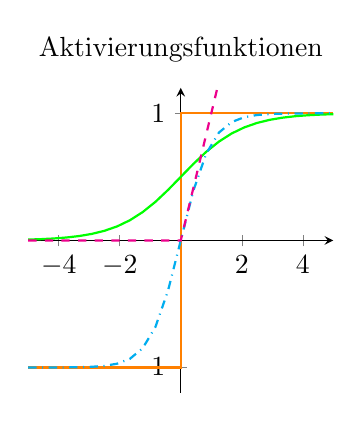
\begin{tikzpicture}
        \begin{axis}[
            width=0.45\textwidth,
            height=0.45\textwidth,
            axis lines=middle,
            xlabel={},
            ylabel={},
            ymin=-1.2, ymax=1.2,
            xmin=-5, xmax=5,
            title= {Aktivierungsfunktionen}
        ]
        % Step function
        \addplot[color=orange, thick] coordinates {
            (-5, -1) (0, -1) (0, 1) (5, 1)};
        % Sigmoid function
        \addplot[color=green, thick] {1 / (1 + exp(-x))};
        % Tanh function
        \addplot[dashdotted, color=cyan, thick] {tanh(x)};
        % ReLU function
        \addplot[thick, color=magenta, dashed] {max(0, x)};
        \end{axis}
    \end{tikzpicture}
    \hspace{0.5cm}
    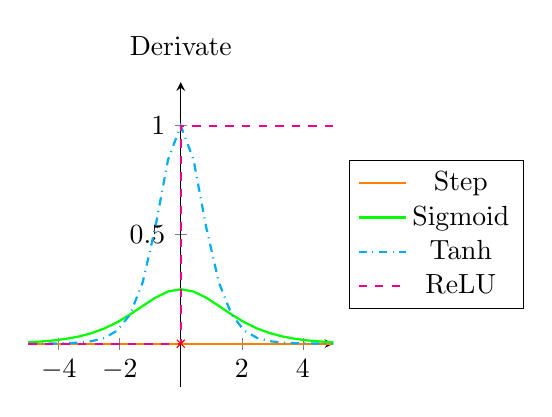
\begin{tikzpicture}
        \begin{axis}[
            width=0.45\textwidth,
            height=0.45\textwidth,
            axis lines=middle,
            xlabel={},
            ylabel={},
            ymin=-0.2, ymax=1.2,
            xmin=-5, xmax=5,
            legend pos= north west,
            title={Derivate},
           legend style={at={(1.05,0.5)}, anchor=west}
        ]
        % Derivative of Step function
        \addplot[color=orange, thick] coordinates {
            (-5, 0) (0, 0) (0, 0) (0.0, 0) (5, 0)
        };
        % Derivative of Sigmoid function
        \addplot[ color=green, thick] {exp(-x) / ((1 + exp(-x))^2)};
        % Derivative of Tanh function
        \addplot[dashdotted, color=cyan, thick] {1 - tanh(x)^2};
        % Derivative of ReLU function
        \addplot[thick, dashed, color=magenta] coordinates {
            (-5, 0) (0, 0) (0, 1) (5, 1)
        };
        \addplot[red, only marks, mark=x] coordinates {(0, 0)}; 
        \legend{Step, Sigmoid, Tanh, ReLU}
        \end{axis}
    \end{tikzpicture}
    \caption{Aktivierungsfunktionen und deren Derivate, nach \citet[S. 292]{Geron:2019}.}
    \label{fig:4.1}
\end{figure}


\subsection{Backpropagation \& Gradientenabstieg}

Die Gewichte eines \ac{dnn} werden durch die Minimierung einer Verlustfunktion (engl. \textit{loss function}) angepasst, um möglichst genaue Vorhersagen zu erzielen. Die Verlustfunktion ist entscheidend für die Optimierung der Modellparameter. (Vgl. \citealt[S. 113]{Geron:2019}). Eine der grundlegenden Verlustfunktionen ist der mittlere quadratische Fehler (engl. \textit{\ac{mse}}): 
\begin{equation}
\begin{aligned}
\label{eq:4.6}
L_{\text{MSE}} = \frac{1}{2n} \sum_{x} \left\| y(x) - \tilde{y} \right\|^2,
\end{aligned}
\end{equation}
wobei \textit{n} die Anzahl der Trainingsbeispiele \(x\) und \( \tilde{y} \) die zugehörigen tatsächlichen Labels darstellt, während \( y(x) \) die Netzwerkausgabe repräsentiert.\\
Der Trainingsprozess beginnt mit der zufälligen Initialisierung der Gewichte, gefolgt von einer iterative Anpassung durch einen Optimierungsprozess zur Minimierung der Verlustfunktion (vgl. \citealt[S. 118]{Geron:2019}). Laut \citet[S. 83-85]{Goodfellow:2017} ist der Gradientenabstieg (engl. \textit{\ac{gd}}), der erstmals von \citet[]{Cauchy:1847} eingeführt wurde, einer der grundlegendsten Optimierungsalgorithmen. Der Algorithmus passt die Netzwerkparameter \(\theta\) entlang des negativen Gradienten der Verlustfunktion an. Die Größe der Anpassung wird durch die Lernrate \(\epsilon\) bestimmt:
\begin{equation}
\begin{aligned}
    \Delta \theta \equiv - \epsilon \nabla_\theta L(\theta).
\end{aligned}
\end{equation}
Im Verlauf jedes Optimierungsschritts werden die Netzwerkparameter gemäß der folgenden Regel aktualisiert:
\begin{equation}
\begin{aligned}
    \theta \leftarrow \theta - \epsilon \nabla_\theta L(\theta).
\end{aligned}
\end{equation}
Bei Anwendung der \ac{mse}-Verlustfunktion \eqref{eq:4.6} ergibt sich die Anpassung der Netzwerkparameter wie folgt:
\begin{equation}
\begin{aligned}
\label{eq:4.9}
    \Delta \theta = - \epsilon \nabla_\theta \left( \frac{1}{2n} \sum_{x} \| y(x) - \tilde{y} \|^2 \right).
\end{aligned}
\end{equation}
In Gleichung \eqref{eq:4.9} wird die Summe über alle Trainingsbeispiele berechnet, weshalb jedes Eingangssignal durch das Netz geleitet werden muss, um die Ausgangssignale \( y(x) \) zu berechnen. Erst im Anschluss kann eine Anpassung der Gewichte durch Gradientenabstieg erfolgen. Insbesondere bei großen Datensätzen ist dies ein rechnerisch aufwändiger Prozess. (Vgl. \citealt[S. 28]{Lang:2023}).\\
Dieses Vorgehen wird durch den Backpropagation-Algorithmus unterstützt, welcher durch \citet[]{Rumelhart:1986} und \citet[]{Rumelhart:1986_} entwickelt wurde. Der Prozess lässt sich in zwei Phasen unterteilen: Im ersten Schritt, dem sogenannten \textit{"`Forward Pass"'}, wird jede Trainingsinstanz durch das Netzwerk geleitet, um Vorhersagen zu treffen. Im sogenannten \textit{"`Reverse Pass"'} wird der durch den Vergleich der Vorhersage mit den tatsächlichen Werten entstandene Fehler durch die Schichten des Netzwerks zurückpropagiert. Auf diese Weise wird der Beitrag jeder Verbindung zum Fehler bestimmt, um die entsprechenden Gewichte anzupassen. Dieser Prozess wird als Gradientenabstiegsschritt (engl. \textit{Gradient Descent step}) bezeichnet, bei dem die Gewichte in kleinen Schritten optimiert werden, um den Fehler zu minimieren. (Vgl. \citealt[S. 291]{Geron:2019}).\\
Der hier beschriebene Algorithmus, der alle Trainingsdaten für jeden Optimierungsschritt verwendet, wird als Batch-Gradientenabstieg (engl. \textit{Batch Gradient Descent}) bezeichnet (vgl. \citealt[S. 122]{Geron:2019}). Obwohl dieser Ansatz präzise ist, kann er bei großen Datensätzen ineffizient sein und führt oft dazu, dass das Modell in lokalen Minima hängen bleibt (vgl. \citealt[S. 119]{Geron:2019}). Daher wurde der Mini-Batch-Gradientenabstieg (engl. \textit{Mini-batch Gradient Descent}) entwickelt, bei dem lediglich ein Teil der Daten in jedem Schritt Berücksichtigung findet, was den Rechenaufwand reduziert und zu einer stabileren Konvergenz führen kann (vgl. \citealt[S. 124-127]{Geron:2019}). Die Anzahl der Beispiele, die den Algorithmen vor jedem Optimierungsschritt vorgelegt werden, die sogenannte Batchgröße (engl. \textit{batch size}), beeinflusst die Optimierungsleistung und senkt die Berechnungsanforderungen (vgl. \citealt[S. 326]{Geron:2019}). \\
Moderne Algorithmen wie der Adam-Optimierer fügen dem Gradientenabstieg einen Impulsterm hinzu, um vergangene Gradienteninformationen in die Parameteraktualisierung einfließen zu lassen. Der Aktualisierungsschritt erfolgt folgendermaßen:
\begin{equation}
\begin{aligned}
\mathbf{m} &\leftarrow \beta \mathbf{m} - \epsilon \nabla_\theta L(\theta) \\
\theta &\leftarrow \theta + \mathbf{m},
\end{aligned}
\end{equation}
wobei \(\mathbf{m}\) der Impulsterm ist und \(\beta\) ein Wert zwischen 0 und 1 darstellt, der die Gewichtung des Impulsterms bestimmt. Die Berücksichtigung früherer Gradienten ermöglicht eine effizientere und robustere Konvergenz als dies bei einfachen Gradientenabstiegsverfahren der Fall ist. (Vgl. \citealt[S. 351-352]{Geron:2019}).

\subsection{Modellparametrisierung \& Generalisierung}

Die Minimierung der Verlustfunktion auf den Trainingsdaten zielt darauf ab, das Modell zu optimieren, indem die Fehler auf den Trainingsdaten reduziert werden. Die Annahme basiert darauf, dass das Modell allgemeine Muster erlernt, welche auf das zugrunde liegende Problem übertragbar sind, sodass auch auf neuen, bisher nicht betrachteten Datensätzen adäquate Resultate erzielt werden. Diese Fähigkeit des Modells, auch auf neuen Daten eine gute Performance zu zeigen, wird als Generalisierung (engl. \textit{generalization}) bezeichnet. Ein niedriger Trainingsfehler (engl. \textit{training error}) indiziert eine effektive Performance des Modells auf den Trainingsdaten, während ein geringer Generalisierungsfehler (engl. \textit{generalization error}) darauf hinweist, dass das Modell seine Leistung auch auf unabhängigen Daten beibehalten kann. Allerdings besteht häufig eine gewisse Spannung zwischen den Zielen der Optimierung und der Generalisierung, da eine Minimierung des Trainingsfehlers nicht zwangsläufig zu einer Verbesserung der Generalisierung führt. Das Ziel ist daher, einen Ausgleich zu finden, um sowohl auf den Trainings- als auch auf den Testdaten gute Ergebnisse zu erzielen. (Vgl. \citealt[S. 128]{Chollet:2021}).\\
\ac{dnn} verfügen über eine signifikante Anzahl an trainierbaren Parametern, die in vielen Fällen eine Größe von Zehntausenden bis zu Millionen aufweisen. Die hohe Anzahl an Parametern ermöglicht dem Modell eine hohe Flexibilität bei der Erfassung und Verarbeitung komplexer Datensätze. (Vgl. \citealt[S. 364]{Geron:2019}). Diese Flexibilität ist auf die Freiheitsgrade (engl. \textit{\ac{dof}}) des Modells zurückzuführen, welche durch die Anzahl der Trainingsparameter definiert werden (vgl. \citet[S. 28]{Geron:2019}). Eine hohe Anzahl an Freiheitsgraden birgt jedoch das Risiko einer Überanpassung (engl. \textit{overfitting}), bei der das Modell spezifische Details der Trainingsdaten anstatt allgemeiner Muster erlernt. Dies kann zu einer Beeinträchtigung der Leistung des Modells auf neuen, ungesehenen Daten führen. (Vgl. \citealt[S. 110-111]{Chollet:2021}). Demgegenüber kann ein Modell, welches über eine unzureichende Anzahl an Freiheitsgraden verfügt, wesentliche Muster nicht adäquat erfassen, was als Unteranpassung (engl. \textit{underfitting}) bezeichnet wird. (Vgl. \citealt[S. 29]{Geron:2019}). Daher ist es von entscheidender Bedeutung, bei der Modellparametrisierung ein ausgewogenes Verhältnis zwischen der Optimierung der Leistung auf den Trainingsdaten und der Minimierung des Generalisierungsfehlers zu finden, um eine adäquate Leistung auf neuen Daten zu gewährleisten (vgl. \citealt[S. 28]{Geron:2019}).\\
Zur Überwachung des Generalisierungsfehlers des Modells während des Trainings wird ein Teil der Trainingsdaten als Validierungsset verwendet. Das unabhängige Set, welches nicht in die Modellanpassung einfließt, findet nach jedem Optimierungsschritt bzw. jeder Trainingsepoche Anwendung, um eine unvoreingenommene Verlustfunktion und weitere Metriken zu berechnen. (Vgl. \citealt[S. 102-104]{Chollet:2021}).\\
Die Generalisierungsdifferenz, definiert als die Abweichung der Modellleistung zwischen Trainings- und Validierungsset, erlaubt eine Beurteilung der Qualität der Generalisierung auf neue, bislang nicht betrachtete Daten. Eine hohe Abweichung kann auf eine Overfitting oder Underfitting hindeuten. Zur Optimierung der Modellleistung wird die Performance auf dem Validierungsset häufig zur Anpassung von Hyperparametern wie der Anzahl der Schichten, Neuronen oder der Lernrate genutzt, da diese direkt die Modellkapazität und Generalisierung beeinflussen. (Vgl. \citealt[S. 29]{Lang:2023}).\\
Für die abschließende Bewertung der Modellleistung wird schließlich ein drittes, unabhängiges Testset verwendet. Das Testset dient der finalen Evaluierung und wird nicht für Training oder Validierung verwendet. Dies gewährleistet eine objektive Beurteilung der Modellleistung. Daher basiert das Training auf drei Datensätzen: dem Trainingsset zur Anpassung der Gewichte, dem Validierungsset zur Überwachung der Generalisierung und dem Testset zur abschließenden Bewertung. (Vgl. \citealt[S. 151-152]{Chollet:2021}).

\subsection{Problemformulierung}

Die Auswahl einer passenden Verlustfunktion stellt einen wesentlichen Aspekt im Rahmen der Modellierung dar. Es existiert eine Vielzahl von Verlustfunktionen, die für spezifische Aufgabenbereiche adaptiert wurden. In der Praxis wird bei der Regression, bei der eine skalare Ausgabe modelliert wird, häufig die \ac{mse}-Verlustfunktion  (\ref{eq:4.6}) verwendet. Im Kontext des Trainings von Klassifikationsmodellen kommt hingegen in der Regel die kategoriale Kreuzentropie (engl. \textit{\ac{cce}}) zum Einsatz:
\begin{align}
    L_\text{CCE} = -\sum_{i=1}^{n} y_i \log(p_i),
\end{align}
wobei \(y_i\) für das wahre Label, \(p_i\) für die Softmax-Wahrscheinlichkeit der Klasse \(i\) und \(n\) für die Gesamtanzahl der Klassen steht. (Vgl. \citealt[S. 101-102]{Chollet:2021}). Die \ac{cce}-Verlustfunktion bestraft falsche Vorhersagen stärker als der \ac{mse},  weshalb sie sich insbesondere für Klassifikationsaufgaben eignet (vgl. \citealt[S. 149]{Geron:2019}).\\
Bei unbalancierten Datensätzen, deren Klassenverteilung eine unausgeglichene Verteilung aufweist, kann die Einführung eines Gewichtungstermins in die Verlustfunktion dazu beitragen, die Repräsentanz unterrepräsentierter Klassen zu verbessern. Dazu wird jeder Summand mit einem Gewichtungsfaktor \(w_i\) multipliziert, sodass unterrepräsentierte Klassen stärker berücksichtigt werden:
\begin{align}
    L_\text{wCCE} = -\sum_{i=1}^{n} w_i y_i \log(p_i).
\end{align}
(Vgl. \citealt[S. 30]{Lang:2023}).

\subsection{Leistungsbewertung} 
Neben der Verlustfunktion ist die Auswahl geeigneter Metriken für die Evaluierung der Modellleistung während der Validierung und des Tests von entscheidender Bedeutung. Diese Metriken spiegeln nicht nur die Genauigkeit des Modells wider, sondern auch dessen Fähigkeit, mit unausgewogenen Datensätzen umzugehen und auf unbekannte Daten zu generalisieren. (Vgl. \citet[S. 34-35]{Tiwari:2022}). \\
Eine Konfusionsmatrix (engl. \textit{\acf{cm}}) stellt ein wesentliches Instrument zur Darstellung der tatsächlichen Labels im Verhältnis zu den prognostizierten Labels dar. Die Darstellung erfolgt in Form einer Matrix, in der die Anzahl der korrekt vorhergesagten positiven Fälle (engl. \textit{\ac{tp}}), der korrekt vorhergesagten negativen Fälle (engl. \textit{\ac{tn}}), der falsch als positiv vorhergesagten Fälle (engl. \textit{\ac{fp}}) sowie der falsch als negativ vorhergesagten Fälle (engl. \textit{\ac{fn}}) angezeigt wird. Aus der \ac{cm} lassen sich mehrere Metriken ableiten, die zur Bewertung von Klassifikationsmodellen für binäre Klassen sowie für Mehrfachklassifikationen verwendet werden können. Die Abbildung \ref{fig:4.2} illustriert eine \ac{cm} für binäre Klassifikationen. Bei einer Mehrklassenklassifikation wie in der Abbildung \ref{fig:4.3} wird die Matrix um die Vorhersagen für jede Klasse gegenüber den tatsächlichen Klassen erweitert, wodurch eine detaillierte Analyse der Modellleistung ermöglicht wird. (Vgl. \citealt[S. 52]{Tiwari:2022}).
\begin{figure}[H]
    \centering
     % Resize the entire tikzpicture
    \resizebox{0.5\textwidth}{!}{ % Scale to 50% of text width
    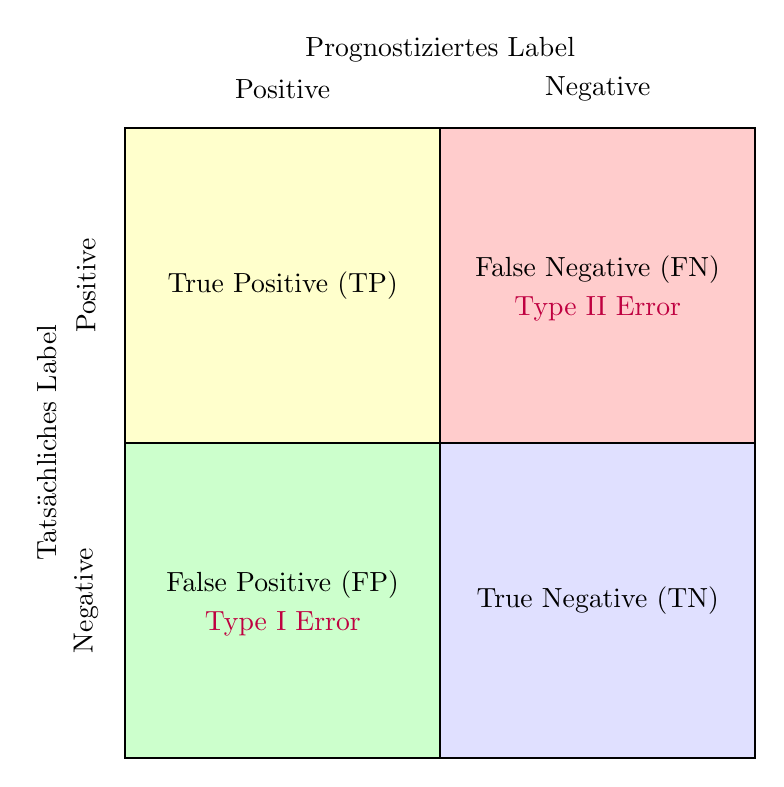
\begin{tikzpicture}
        % Definiere die Farben für die Felder
        \definecolor{tpcolor}{RGB}{255, 255, 204}
        \definecolor{fncolor}{RGB}{255, 204, 204}
        \definecolor{fpcolor}{RGB}{204, 255, 204}
        \definecolor{tncolor}{RGB}{224, 224, 255}

        % Zeichne die Zellen
        \fill[tpcolor] (0, 0) rectangle (4, -4);
        \fill[fncolor] (4, 0) rectangle (8, -4);
        \fill[fpcolor] (0, -4) rectangle (4, -8);
        \fill[tncolor] (4, -4) rectangle (8, -8);

        % Zeichne die Begrenzungslinien
        \draw[thick] (0, 0) rectangle (8, -8);
        \draw[thick] (0, -4) -- (8, -4);
        \draw[thick] (4, 0) -- (4, -8);

        % Beschriftung der Zellen
        \node at (2, -2) {True Positive (TP)};
        \node at (6, -1.8) {False Negative (FN)};
        \node at (6, -2.3){\textcolor{purple}{Type II Error}}; 
        \node at (2, -5.8) {False Positive (FP)};
        \node at (2, -6.3){\textcolor{purple}{Type I Error}}; 
        \node at (6, -6) {True Negative (TN)};

        % Beschriftung der Achsen
        \node[rotate=90] at (-1, -4) {Tatsächliches Label};
        \node at (4, 1) {Prognostiziertes Label};
        
        % Beschriftung der Klassen
        \node at (2, 0.5) {Positive};
        \node at (6, 0.5) {Negative};
        \node[rotate=90] at (-0.5, -2) {Positive};
        \node[rotate=90] at (-0.5, -6) {Negative};
        
        % Überschrift der Matrix
       % \node at (4, 2) {\textbf{Confusion Metric}};

        % Pfeile für die Achsen
        %\draw[thick,->] (-1.5, -8) -- (-1.5, 0);
        %\draw[thick,->] (0, 1.5) -- (8, 1.5);
    \end{tikzpicture}
    }
    \caption{Binäre \ac{cm}, nach \citet[S. 52]{Tiwari:2022}.}
    \label{fig:4.2}
\end{figure}

\setlength{\leftmargini}{5pt} % Setzt die Einrückung auf 0
\begin{itemize}
  \item \textbf{\textit{Accuracy}}:\\
  Die Accuracy (Genauigkeit) eines Modells gibt das Verhältnis zwischen der Gesamtzahl der vom Modell richtig prognostizierten Labels und der Gesamtzahl der Labels an.
   \begin{equation}
  \begin{aligned}
      Accuracy = \frac{\text{TP} + \text{TN}}{\text{TP} + \text{TN} + \text{FP} + \text{FN}}
  \end{aligned}
  \end{equation}
  In Fällen einer unbalancierten Klassenverteilung kann die Accuracy jedoch irreführende Ergebnisse liefern, da sie durch überrepräsentierte Klassen dominiert werden kann (vgl. \citealt[S. 56]{Tiwari:2022}).
  \item \textbf{\textit{\ac{tpr}}}:\\
  Die \ac{tpr} beschreibt das Verhältnis der korrekt prognostizierten positiven Labels zur Gesamtzahl der tatsächlichen positiven Labels. Die \ac{tpr} ist auch als \textbf{\textit{Recall}} oder \textbf{\textit{Sensitivity}} bekannt.
   \begin{equation}
  \begin{aligned}
      TPR = \frac{\text{TP}}{\text{TP} + \text{FN}}
  \end{aligned}
  \end{equation}
   \item \textbf{\textit{\ac{tnr}}}:\\
  Die \ac{tnr} beschreibt das Verhältnis der korrekt prognostizierten negativen Labels zur Gesamtzahl der tatsächlichen negativen Labels. Eine andere Bezeichnung für \ac{tnr} ist die \textbf{\textit{Specificity}}. 
   \begin{equation}
  \begin{aligned}
      TNR = \frac{\text{TN}}{\text{FP} + \text{TN}}
  \end{aligned}
  \end{equation}
  Im Rahmen binärer Klassifikationsaufgaben, wie sie in zahlreichen klinischen Tests zum Einsatz gelangen, sind die Metriken Sensitivität und Spezifität von entscheidender Bedeutung. Sie stehen proportional zur Güte des Modells (vgl. \citealt[S. 30-31]{Lang:2023}). 
 \item \textbf{\textit{\ac{fnr}}}:\\
 Die \ac{fnr} stellt das Verhältnis der falsch vorhergesagten positiven Labels zur Gesamtzahl der tatsächlichen positiven Labels dar.
   \begin{equation}
   \begin{aligned}
      FNR = \frac{\text{FN}}{\text{TP} + \text{FN}}
  \end{aligned}
  \end{equation}
   \item \textbf{\textit{\ac{fpr}}}:\\
 Die \ac{fpr} gibt das Verhältnis der falsch vorhergesagten negativen Labels zur Gesamtzahl der tatsächlichen negativen Labels an.
    \begin{equation}
   \begin{aligned}
      FPR = \frac{\text{FP}}{\text{FP} + \text{TN}}
  \end{aligned}
  \end{equation}
  Die Güte des Modells steht in inversem Verhältnis zu den Metriken \ac{tnr} und \ac{fpr} (vgl. \citealt[S. 57-58]{Tiwari:2022}).
  \item \textbf{\textit{Precision}}:\\
 Die Precision gibt an, wie viele positive Labels im Verhältnis zu allen positiv prognostizierten Labels richtig prognostiziert wurden. 
    \begin{equation}
   \begin{aligned}
      Precision = \frac{\text{TP}}{\text{TP} + \text{FP}}
  \end{aligned}
  \end{equation}
  Es besteht eine negative Korrelation zwischen Precision und Recall (\ac{tpr}) (vgl. \citealt[S. 60-61]{Tiwari:2022}).
   \item \textbf{\textit{F1-Score}}:\\
Der F1-Score stellt ein harmonisches Mittel von Precision und Recall dar, welches eine Balance zwischen beiden Metriken bietet.\\
\begin{equation}
    \begin{aligned}
        F_1 &= \frac{2}{\text{Precision}^{-1} + \text{Recall}^{-1}}
        &= 2\cdot \frac{\text{Precision} \cdot \text{Recall}}{\text{Precision} + \text{Recall}}
    \end{aligned}
\end{equation}
 Der F1-Score gewichtet niedrige Werte deutlich stärker als hohe Werte. Folglich wird ein hoher F1-Score nur bei hohen Werten für Recall und Precision erreicht. (Vgl. \citealt[S. 61]{Tiwari:2022}).
\end{itemize}
Im Rahmen einer Mehrklassenklassifikation erfolgt die Berechnung von Precision, Recall und F1-Score für jede Klasse. Die Ergebnisse werden in einem Klassifikationsbericht (engl. \textit{\acf{cr}}) dargestellt. Die nachfolgende Tabelle \ref{tab:4.1} veranschaulicht dies anhand von einem \ac{cr} für \(n\) = 4 Klassen und insgesamt 1550 Datenpunkte. Der jeweilige Support gibt die Anzahl der beobachteten Datenpunkte bei der jeweiligen Metrik an.  Im Folgenden werden die verschiedenen Verfahren zur Berechnung der Metriken erläutert, nämlich Micro Average, Macro Average und Weighted Average. (Vgl. \citealt[S. 6]{Grandini:2020}).

% Definiere die Farben
\definecolor{tpcolor}{RGB}{255, 255, 204}
\definecolor{fncolor}{RGB}{255, 204, 204}
\definecolor{fpcolor}{RGB}{204, 255, 204}
\definecolor{tncolor}{RGB}{224, 224, 255}

% Rechte Tabelle: Konfusionsmatrix mit Werten
\begin{figure}[ht]
    \centering
     \resizebox{0.7\textwidth}{!}{ % Scale to 70% of text width
    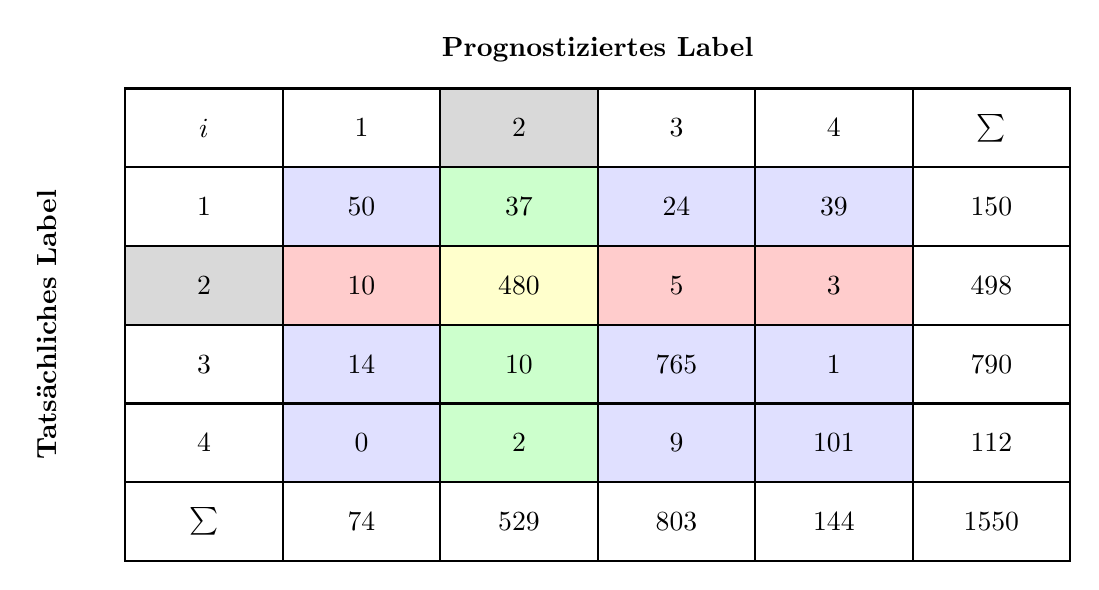
\begin{tikzpicture}

        % Rechte Tabelle
        \node at (12, 4.5) {\textbf{Prognostiziertes Label}};
        \node[rotate=90] at (5, 1) {\textbf{Tatsächliches Label}};

        % Horizontale Kopfzeile
        \draw[thick, fill=white] (6, 3) rectangle (8, 4);
        \node at (7, 3.5) {\(i\)};
        \draw[thick, fill=white] (8, 3) rectangle (10, 4);
        \node at (9, 3.5) {1};
        \draw[thick, fill=Black!15] (10, 3) rectangle (12, 4);
        \node at (11, 3.5) {2};
        \draw[thick, fill=white] (12, 3) rectangle (14, 4);
        \node at (13, 3.5) {3};
        \draw[thick, fill=white] (14, 3) rectangle (16, 4);
        \node at (15, 3.5) {4};
        \draw[thick, fill=white] (16, 3) rectangle (18, 4);
        \node at (17, 3.5) {\(\sum\)};

        % Vertikale Kopfzeile
        \draw[thick, fill=white] (6, 2) rectangle (8, 3);
        \node at (7, 2.5) {1};
        \draw[thick, fill=Black!15] (6, 1) rectangle (8, 2);
        \node at (7, 1.5) {2};
        \draw[thick, fill=white] (6, 0) rectangle (8, 1);
        \node at (7, 0.5) {3};
        \draw[thick, fill=white] (6, -1) rectangle (8, 0);
        \node at (7, -0.5) {4};
        \draw[thick, fill=white] (6, -2) rectangle (8, -1);
        \node at (7, -1.5) {\(\sum\)};

        % Zellen - Zeile 1
        \draw[thick, fill=tncolor] (8, 2) rectangle (10, 3); % TN
        \node at (9, 2.5) {50};

        \draw[thick, fill=fpcolor] (10, 2) rectangle (12, 3); % FP
        \node at (11, 2.5) {37};

        \draw[thick, fill=tncolor] (12, 2) rectangle (14, 3); % TN
        \node at (13, 2.5) {24};

        \draw[thick, fill=tncolor] (14, 2) rectangle (16, 3); % TN
        \node at (15, 2.5) {39};

        \draw[thick, fill=white] (16, 2) rectangle (18, 3); % Zeilensumme
        \node at (17, 2.5) {150};

        % Zellen - Zeile 2
        \draw[thick, fill=fncolor] (8, 1) rectangle (10, 2); % FN
        \node at (9, 1.5) {10};

        \draw[thick, fill=tpcolor] (10, 1) rectangle (12, 2); % TP
        \node at (11, 1.5) {480};

        \draw[thick, fill=fncolor] (12, 1) rectangle (14, 2); % FN
        \node at (13, 1.5) {5};

        \draw[thick, fill=fncolor] (14, 1) rectangle (16, 2); % FN
        \node at (15, 1.5) {3};

        \draw[thick, fill=white] (16, 1) rectangle (18, 2); % Zeilensumme
        \node at (17, 1.5) {498};

        % Zellen - Zeile 3
        \draw[thick, fill=tncolor] (8, 0) rectangle (10, 1); % TN
        \node at (9, 0.5) {14};

        \draw[thick, fill=fpcolor] (10, 0) rectangle (12, 1); % FP
        \node at (11, 0.5) {10};

        \draw[thick, fill=tncolor] (12, 0) rectangle (14, 1); % TN
        \node at (13, 0.5) {765};

        \draw[thick, fill=tncolor] (14, 0) rectangle (16, 1); % TN
        \node at (15, 0.5) {1};

        \draw[thick, fill=white] (16, 0) rectangle (18, 1); % Zeilensumme
        \node at (17, 0.5) {790};

        % Zellen - Zeile 4
        \draw[thick, fill=tncolor] (8, -1) rectangle (10, 0); % TN
        \node at (9, -0.5) {0};

        \draw[thick, fill=fpcolor] (10, -1) rectangle (12, 0); % FP
        \node at (11, -0.5) {2};

        \draw[thick, fill=tncolor] (12, -1) rectangle (14, 0); % TN
        \node at (13, -0.5) {9};

        \draw[thick, fill=tncolor] (14, -1) rectangle (16, 0); % TN
        \node at (15, -0.5) {101};

        \draw[thick, fill=white] (16, -1) rectangle (18, 0); % Zeilensumme
        \node at (17, -0.5) {112};

        % Spaltensummen
        \draw[thick, fill=white] (8, -2) rectangle (10, -1);
        \node at (9, -1.5) {74};

        \draw[thick, fill=white] (10, -2) rectangle (12, -1);
        \node at (11, -1.5) {529};

        \draw[thick, fill=white] (12, -2) rectangle (14, -1);
        \node at (13, -1.5) {803};

        \draw[thick, fill=white] (14, -2) rectangle (16, -1);
        \node at (15, -1.5) {144};

        \draw[thick, fill=white] (16, -2) rectangle (18, -1);
        \node at (17, -1.5) {1550};

    \end{tikzpicture}
    }
 \resizebox{0.5\textwidth}{!}{ % Scale to 50% of text width
    % Legende
    \vspace{0.5cm}
    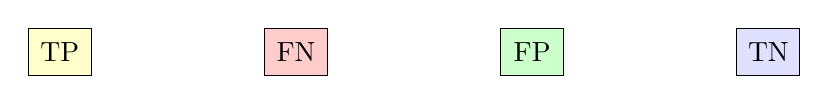
\begin{tikzpicture}
    
    \draw[fill=tpcolor] (1, -0.3) rectangle (1.8, 0.3);
    \node at (1.4, 0) {TP};
    
    \draw[fill=fncolor] (4, -0.3) rectangle (4.8, 0.3);
    \node at (4.4, 0) {FN};
    
    \draw[fill=fpcolor] (7, -0.3) rectangle (7.8, 0.3);
    \node at (7.4, 0) {FP};
    
    \draw[fill=tncolor] (10, -0.3) rectangle (10.8, 0.3);
    \node at (10.4, 0) {TN};
\end{tikzpicture}
}
    \caption{Mehrklassen-\ac{cm} mit Klasse \colorbox{Black!20}{2} als Bezugsklasse, nach \citet[S. 6]{Grandini:2020}.}
    \label{fig:4.3}
\end{figure}

% Classification Report
\begin{table}[H]
\centering
 \resizebox{0.7\textwidth}{!}{ % Scale to 70% of text width
\begin{tabular}{||c||c|c|c|c||}
\hline
\textbf{\(i\)} & \textbf{Precision} & \textbf{Recall} & \textbf{F1-Score} & \textbf{Support} \\
\hline \hline
1 & 0.68 & 0.33 & 0.44 & 150 \\\hline
2 & 0.91 & 0.96 & 0.94 & 498 \\\hline
3 & 0.95 & 0.97 & 0.96 & 790 \\\hline
4 & 0.70 & 0.90 & 0.79 & 112 \\\hline
\textbf{Accuracy} & \multicolumn{3}{c|}{0.90} &1550 \\\hline
\textbf{Macro Avg} & 0.81 & 0.79 & 0.78 & 1550 \\\hline
\textbf{Weighted Avg} & 0.89 & 0.90 & 0.89 & 1550 \\\hline
\end{tabular}
}
\caption{\ac{cr} basierend auf der \ac{cm} in Abbildung \ref{fig:4.3}.}
\label{tab:4.1}
\end{table}

\begin{itemize}
    \item \textbf{\textit{Micro Average}}:\\
    Der Micro Average berechnet die Gesamtperformance eines Modells über alle Klassen hinweg, indem die \ac{tp}, \ac{fp} und \ac{fn} aller Klassen summiert werden, bevor Precision, Recall und der F1-Score ermittelt werden. Diese Vorgehensweise gewährleistet eine gleichwertige Gewichtung aller Instanzen, unabhängig von der Klassengröße, was insbesondere bei ungleich großen Klassen von Vorteil ist. 
    \begin{equation}
    \begin{aligned}
        Micro\ Average\ Precision &= \frac{\sum_{i=1}^{n} \text{TP}_i}{\sum_{i=1}^{n} \text{Total Column}_i}
        &=\frac{\sum_{i=1}^{n} \text{TP}_i}{\text{Grand Total}}
    \end{aligned}
     \end{equation}
     \begin{equation}
    \begin{aligned}
        Micro\ Average\ Recall &= \frac{\sum_{i=1}^{n} \text{TP}_i}{\sum_{i=1}^{n} \text{Total Row}_i}
        &=\frac{\sum_{i=1}^{n} \text{TP}_i}{\text{Grand Total}}
    \end{aligned}
     \end{equation}
     \begin{equation}
    \begin{aligned}
        Micro\ Average\ F_1 =\frac{\sum_{i=1}^{n} \text{TP}_i}{\text{Grand Total}}
    \end{aligned}
     \end{equation}
     Da die Werte von Precision, Recall und F1-Score auf den aggregierten \ac{tp} basieren, sind sie im Micro Average identisch und spiegeln die Accuracy des Modells wider. Demgemäß wird bei dem \ac{cr} lediglich der Wert der Accuracy, wie in Tabelle \ref{tab:4.1} dargestellt, ausgewiesen. (Vgl. \citealt[S. 7-8]{Grandini:2020}).
    \item \textbf{\textit{Macro Average}}:\\
    Der Macro Average berechnet die Precision, den Recall und den F1-Score für jede Klasse \(i\) separat und bildet anschließend den Durchschnitt der einzelnen Werte.
     \begin{equation}
    \begin{aligned}
        Macro\ Average\ Precision = \frac{1}{n} \sum_{i=1}^{n} \text{Precision}_i
    \end{aligned}
     \end{equation}
     \begin{equation}
     \begin{aligned}
       Macro\ Average\ Recall = \frac{1}{n} \sum_{i=1}^{n} \text{Recall}_i
    \end{aligned}
     \end{equation}
     \begin{equation}
     \begin{aligned}
        Macro\ Average\ F_1 = \frac{1}{n} \sum_{i=1}^{n} \text{F}_1i
    \end{aligned}
     \end{equation}
   Der Macro Average gewichtet jede Klasse unabhängig von ihrer Größe gleich, wodurch die Leistung des Modells in allen Klassen gleichermaßen berücksichtigt wird. Dies ist insbesondere von Vorteil, wenn auch kleine Klassen mit wenigen Datenpunkten gleichwertig einbezogen werden sollen. (Vgl. \citealt[S. 6-7]{Grandini:2020}).
    \item \textbf{\textit{Weighted Average}}:\\
     Der Weighted Average berücksichtigt sowohl die Performance der einzelnen Klassen als auch den Support in jeder Klasse. In der Folge werden für jede Klasse Precision, Recall sowie F1-Score berechnet. Dabei findet eine Gewichtung nach dem Support pro Klasse.
     \begin{equation}
    \begin{aligned}
        Weighted\ Average\ Precision = \frac{\sum_{i=1}^{n} (\text{Precision}_i \cdot \text{Support}_i)}{\sum_{i=1}^{n} \text{Support}_i} 
    \end{aligned}
    \end{equation}
     \begin{equation}
     \begin{aligned}
       Weighted\ Average\ Recall = \frac{\sum_{i=1}^{n} (\text{Recall}_i \cdot \text{Support}_i)}{\sum_{i=1}^{n} \text{Support}_i} 
    \end{aligned}
    \end{equation}
     \begin{equation}
     \begin{aligned}
       Weighted\ Average\ F_1 = \frac{\sum_{i=1}^{n} (\text{F}_1i \cdot \text{Support}_i)}{\sum_{i=1}^{n} \text{Support}_i} 
    \end{aligned}
    \end{equation}
    Der Weighted Average berücksichtigt die Klassengröße und ist somit bei der Anwendung des Modells auf Datensätze mit unbalancierten Klassenverteilungen vorteilhaft. Dabei tragen Klassen mit einem höheren Support stärker zum Gesamtwert bei. (Vgl. \citealt[S. 68]{Tiwari:2022} sowie \citealt[S. 9]{Wang:2023}).
\end{itemize}

\subsection{Regularisierungs- \& Augmentierungstechniken}

Bei Aufgaben, bei denen große Datensätze nur schwer zu erlangen sind, ist das Risiko eines Overfittings des Netzwerks an den Trainingsdaten mit der Größe des Netzwerks signifikant erhöht. Zur Verhinderung vom Overfitting werden in der Praxis zwei gängige Ansätze verfolgt: Regularisierung und Datenaugmentation. (Vgl. \citealt[S. 31]{Lang:2023}).\\
Im Rahmen der Regularisierung wird die Anpassungsfähigkeit des Modells an die Trainingsdaten gezielt reduziert, was eine bessere Generalisierung auf unbekannte Daten zur Folge hat und zu einer verbesserten Leistung auf Validierungsdaten führen kann (vgl. \citealt[S. 146]{Chollet:2021}). Eine übliche Methode ist die Gewichtsregularisierung, bei der ein zusätzlicher Term zur Verlustfunktion hinzugefügt wird, der große Werte für die Modellparameter bestraft (vgl. \citealt[S. 148-149]{Chollet:2021}).Die L1-Regularisierung resultiert in der Regel in sparsamen Modellen, indem viele Parameter auf Null gesetzt werden, was dazu führt, dass das Modell nur die relevantesten Merkmale lernt (vgl. \citealt[S. 137-138]{Geron:2019}). Im Gegensatz dazu reduziert die L2-Regularisierung die Größe aller Parameter, wodurch übermäßig große Gewichtungen vermieden werden und das Modell weniger anfällig für Overfitting wird (vgl. \citealt[S. 135]{Geron:2019}). Dies impliziert eine Limitation der Modellwahl und eine Verhinderung der exakten Anpassung an die Trainingsdaten. Es lassen sich zwei Hauptarten unterscheiden:
\begin{enumerate}
    \item[] L1-Regularisierung: 
\begin{equation}
    \begin{aligned}
        Loss \rightarrow Loss + \lambda \sum_{j} |\theta_i|,
    \end{aligned} 
    \end{equation}
     wobei \(\theta_i\) die trainierbaren Netzparameter bezeichnet, während \(\lambda\) die Auswirkungen des Regularisierungsterms steuert.
     \item[] L2-Regularisierung: 
\begin{equation}
    \begin{aligned}
        Loss \rightarrow Loss + \lambda \sum_{j} \theta_i^2.
    \end{aligned} 
    \end{equation}     
\end{enumerate}
Die Entscheidung zwischen L1 und L2 hängt vom Problem ab. L1 erweist sich insbesondere bei sparsamen Modellen mit wenigen relevanten Parametern als vorteilhaft. Bei gleichmäßig verteilten Gewichten ist eine L2-Regulierung zu bevorzugen. (Vgl. \citealt[S. 138-139]{Geron:2019} sowie \citealt[S. 236]{Goodfellow:2017}). \\
Die Anwendung der Gewichtsregularisierung ist insbesondere bei kleinen \ac{dl}-Modellen von Nutzen. Bei großen \ac{dl}-Modellen, die häufig eine hohe Anzahl an Parametern aufweisen, zeigt sich, dass die Einführung von Beschränkungen für Gewichtswerte durch Gewichtsregularisierung einen vergleichsweise geringen Einfluss auf die Modellkapazität hat. In diesen Fällen werden daher andere Regularisierungstechniken wie Dropout eingesetzt. (Vgl. \citealt[S. 150]{Chollet:2021}).\\
Im Rahmen des Dropouts werden Neuronen zufällig ausgewählt, was deren Ausschluss aus dem Optimierungsprozess zur Folge hat. Dies resultiert in einer Reduktion der Speicherkapazität einzelner Neuronen für spezifische Datenpunkte, wodurch ein Overfitting verhindert wird. Der Vorteil von Dropout besteht in der Induktion eines Ensemble-Effekts, da während des Trainings verschiedene Teilmodelle mit zufälligen neuronalen Konfigurationen generiert werden, was die Generalisierungsfähigkeit erhöht. (Vgl. \citealt[S. 365-367]{Geron:2019}).
\\
Die Datenaugmentation bezeichnet eine Methode der künstlichen Vergrößerung von Datensätzen, welche durch Modifikationen der Trainingsdaten erfolgt. In der Bildverarbeitung finden Techniken wie zufällige Rotationen, Spiegelungen, Zoom, Zuschneiden, Hinzufügen von Rauschen sowie Anpassungen von Helligkeit, Kontrast und Sättigung Anwendung. Die genannten Transformationen erhöhen die Robustheit des Modells, da dieses lernt, zugrundeliegende Muster in Bildern unabhängig von den genannten Variationen zu erkennen. Dies führt nicht nur zu einer Reduktion des Risikos eines Overfittings, sondern auch zu einer Verbesserung der allgemeinen Leistungsfähigkeit des Modells. (Vgl. \citealt[S. 465]{Geron:2019}).\\
Insbesondere in Szenarien, die durch limitierte und unausgewogene Datensätze gekennzeichnet sind, erweist sich die Datenaugmentation als vorteilhaft. Die Anwendung von Datenaugmentation ermöglicht es Modellen, Merkmale aus unterschiedlichen Perspektiven und unter variierenden Lichtbedingungen besser zu erkennen, was zu einer Erhöhung der Klassifikationsgenauigkeit beiträgt. Des Weiteren unterstützt sie das Erlernen algorithmischer Vorannahmen über Bildinvarianten, was insbesondere bei der Analyse medizinischer Bilddaten wichtig sein könnte. (Vgl. \citealt[S. 31-32; 48]{Lang:2023}).\\
In der medizinischen Bildverarbeitung sind mit der Datenaugmentation jedoch spezifische Herausforderungen verbunden. Transformationsprozesse wie Rotation oder Zuschneiden können die diagnostische Aussagekraft von Daten beeinträchtigen. Dies kann durch eine fehlerhafte Labelzuweisung oder eine Veränderung kritischer Details bedingt sein. Diese Modifikationen führen zu einer Einschränkung der klinischen Anwendbarkeit der augmentierten Daten. Des Weiteren weisen medizinische Bilder häufig eine höhere Variabilität auf als lediglich geometrische und helligkeitsbezogene Unterschiede. Dies begrenzt die Effektivität herkömmlicher Augmentationstechniken. Fortgeschrittene Ansätze wie Generative Adversarial Networks (GANs) eröffnen vielversprechende Möglichkeiten zur Generierung synthetischer Daten. Allerdings ist zu berücksichtigen, dass GANs eine hohe Anzahl an Ausgangsdaten sowie einen umfassenden Modellierungsaufwand erfordern. Zudem zeigt sich in der Praxis, dass die von GANs erzeugte Bildqualität häufig nicht den Anforderungen klinischer Anwendungen genügt. (Vgl. \citealt[S. 9; 27]{Shorten:2019}).

\subsection{Konvolutionale neuronale Netze}

Konvoultionale neuronale Netze (engl. \textit{\acf{cnn}}) stellen eine bedeutende Architektur von \ac{dl}-Modellen dar, die insbesondere für die Verarbeitung und Analyse von Bilddaten zum Einsatz kommt (vgl. \citealt[S. 445]{Geron:2019}). Im Gegensatz zu traditionellen \ac{mlp} ist die Verarbeitung von Daten durch \ac{cnn} in ihrem natürlichen zweidimensionalen (2D) Format möglich, wodurch die räumlichen Beziehungen zwischen den Pixeln erhalten bleiben (vgl. \citealt[S. 448]{Geron:2019}). Im Falle von \ac{mlp} erfolgt eine Umwandlung der Eingabebilder in einen eindimensionalen (1D) Vektor, was zu einer signifikanten Vergrößerung der Eingabegrößen und einer Vielzahl trainierbarer Parameter führt (vgl. \citealt[S. 447-448]{Geron:2019}). Diese Vorgehensweise erweist sich für die Verarbeitung von Bildern jedoch als suboptimal, da \ac{mlp}s keine Translationsinvarianz aufweisen, was bedeutet, dass Muster nicht erkannt werden können, wenn sie sich an verschiedenen Positionen im Bild befinden (vgl. \citealt[S. 203]{Chollet:2021}). \\
\ac{cnn}s beheben diese Probleme durch die Anwendung von Konvolutionsoperationen (engl. \textit{convolutional operations}) , welche von der Struktur des visuellen Kortex im Gehirn inspiriert sind. Die Studien von \citet[]{Hubel:1959}, \citet[]{Hubel:1959_} und \citet[]{Hubel:1968} führten zu der Erkenntnis,  dass der visuelle Kortex aus Schichten mit hierarchischer Struktur besteht. Eine Vielzahl von Neuronen im visuellen Kortex weist ein kleines lokales rezeptives Feld (engl. \textit{local receptive field}) auf, welches lediglich auf visuelle Stimuli in einem begrenzten Bereich des Gesichtsfelds reagiert. In den frühen Schichten werden einfache Merkmale wie Kanten erkannt, während die tieferen Schichten diese zu komplexeren Formen und letztlich zu vollständigen Objekten kombinieren. Die genannten Erkenntnisse führten zunächst zur Anwendung von manuell erstellten Filtern zur Merkmalsextraktion aus Bilddaten und schließlich zur Entwicklung von \ac{cnn}s. (Vgl. \citealt[S. 446-447]{Geron:2019}).\\
Konvolutionale Schichten (engl. \textit{convolutional layers}) stellen die zentralen Bausteine eines \ac{cnn}s dar. Im Gegensatz zu vollständig verbundenen Schichten weisen Neuronen in den konvolutionalen Schichten lediglich eine geringe Verbindungsstärke zu einem kleinen Bereich der Eingabe auf, dem sogenannten rezeptiven Feld. Infolgedessen können in den initialen Schichten einfache Charakteristika wie Kanten identifiziert und in den nachfolgenden Schichten zu komplexeren Mustern kombiniert werden. Dies trägt maßgeblich zur hohen Effizienz von \ac{cnn}s bei der Bearbeitung von Bilddaten bei, da die visuelle Welt prinzipiell räumlich hierarchisch ist. Um die Schichtgröße konstant zu halten, wird häufig Zero Padding angewendet, bei dem Nullen an den Eingaberändern hinzugefügt werden. Der Stride gibt an, wie stark sich das rezeptive Feld von einem Schritt zum nächsten verschiebt, und ermöglicht es, die Modellkomplexität zu verringern, indem große Eingaben zu kleineren Ausgabeschichten verbunden werden. (Vgl. \citealt[S. 448-449]{Geron:2019}).\\
Ein Filter, auch Konvolutionskern genannt, besteht aus den Gewichtungen eines Neurons und kann als kleines Bild in der Größe des rezeptiven Feldes dargestellt werden. Ein Beispiel wäre ein 3×3-Filter, bei dem nur die mittlere vertikale Linie mit Einsen gefüllt ist, während der Rest Nullen enthält. Dieser Filter aktiviert nur das zentrale vertikale Merkmal in einem Bild, während andere Bereiche des Bildes ignoriert werden. Ein anderer Filter könnte in ähnlicher Weise nur horizontale Linien erkennen. Wenn alle Neuronen in einer Schicht den gleichen Filter verwenden, erzeugen sie eine Merkmalskarte (engl. \textit{feature map}), die die aktivierten Bildbereiche hervorhebt. Während des Trainings lernen Konvolutionale Schichten automatisch, welche Filter am besten geeignet sind, um bestimmte Merkmale in einem Bild zu erkennen, und kombinieren diese in den oberen Schichten zu komplexeren Mustern. Dieser Lernprozess ermöglicht es \ac{cnn}s, immer abstraktere Darstellungen der Bilddaten zu entwickeln. (Vgl. \citealt[S. 450]{Geron:2019}).\\
Pooling-Schichten (engl. \textit{pooling layer}) in \ac{cnn}s weisen eine ähnliche Funktionsweise wie konvolutionale Schichten auf. Auch hier ist jedes Neuron mit einer begrenzten Anzahl von Neuronen der vorherigen Schicht verbunden, wobei diese in einem kleinen rezeptiven Feld liegen. Im Gegensatz zu konvolutionalen Schichten verfügen Pooling-Neuronen nicht über Gewichte, sondern aggregieren die Eingaben durch eine Aggregationsfunktion wie beispielsweise den Max- oder Mittelwert. In der Praxis findet vornehmlich das Max-Pooling Anwendung, bei dem lediglich der jeweils höchste Wert aus jedem rezeptiven Feld an die nachfolgende Schicht weitergeleitet wird, während die übrigen Werte verworfen werden. (Vgl. \citealt[S. 457]{Geron:2019}).\\ 
Die Verwendung von Max-Pooling-Schichten führt zu einer Reduktion der Rechenzeit, des Speicherbedarfs sowie der Anzahl der Parameter. Zudem wird eine gewisse Invarianz gegenüber kleinen Verschiebungen eingeführt. Dadurch wird das Modell weniger anfällig für kleine Verschiebungen in den Bilddaten, was die Generalisierungsfähigkeit erhöht. Zudem bietet das Max-Pooling eine begrenzte Rotations- und Skalierungsinvarianz, was insbesondere bei Klassifikationsaufgaben vorteilhaft ist, bei denen die Vorhersagen von diesen Details unabhängig sein sollen. (Vgl. \citealt[S. 457-458]{Geron:2019}).\\
Die Architektur von \ac{cnn}s umfasst in der Regel mehrere konvolutionale Schichten (+ ReLUs) und Pooling-Schichten, gefolgt von vollständig verbundenen Schichten, welche die extrahierten Merkmale verarbeiten und letztlich zur Klassifikation genutzt werden. Abbildung \ref{fig:4.7} zeigt die Architekur eines \ac{cnn}s. (Vgl. \citealt[S. 460-461]{Geron:2019}).
\begin{figure}[H]
    \centering 
    \includegraphics[width=0.9\textwidth]{BA/Abbildungen/CNN Architektur.jpg} % Bild einfügen, anpassen der Breite
    \caption{Architektur eines \ac{cnn}s, entnommen aus \citet[S. 461]{Geron:2019}.} % Beschriftung der Abbildung
    \label{fig:4.7} % Label für Referenz
\end{figure}
Zusammenfassend lässt sich festhalten, dass die Verarbeitung dreidimensionaler Daten durch \ac{cnn}s möglich ist, insbesondere im Kontext medizinischer Bildgebungsverfahren wie \ac{mrt}- oder \ac{ct}-Scans. In diesen Fällen erfolgt nicht lediglich eine Stapelung der Merkmalskarten in zwei Dimensionen (Höhe und Breite), sondern ebenfalls in der dritten Dimension, wodurch die räumlichen Informationen eines Volumendatensatzes berücksichtigt werden. Die gleichzeitige Verwendung mehrerer Merkmalskarten erlaubt die Extraktion verschiedener Aspekte eines Bildvolumens. Dies ermöglicht es \ac{cnn}s, komplexe 3D-Strukturen zu erkennen und wichtige Muster in dreidimensionalen Daten an unterschiedlichen Positionen mit hoher Effizienz zu verarbeiten. Diese Netze sind speziell darauf ausgelegt, Volumendaten in verschiedenen Schichten hierarchisch zu verarbeiten und zu abstrahieren. Diese Eigenschaft erweist sich insbesondere in der medizinischen Bildgebung als vorteilhaft, da dort eine genaue Erkennung und Segmentierung von Strukturen über mehrere Schichten hinweg erforderlich ist. (Vgl. \citealt[S. 451]{Geron:2019} sowie \citealt[S. 35]{Lang:2023}).

\subsection{Segmentierungsnetze}

\ac{dl}-Modelle finden neben der Klassifikation auch bei der Bildsegmentierung Anwendung. Es existieren zwei Hauptkategorien der Segmentierung: die semantische Segmentierung (engl. \textit{semantic segmentation}) und die Instanzsegmentierung (engl. \textit{instance segmentation}). Im Rahmen der semantischen Segmentierung erfolgt eine pixelweise Klassifikation von Bildbereichen in vordefinierte Kategorien, wobei eine weitere Differenzierung von Objekten derselben Klasse nicht stattfindet. Im Gegensatz dazu erfolgt bei der Instanzsegmentierung eine separate Segmentierung verschiedener Objekte derselben Klasse. (Vgl. \citealt[S. 231-232]{Chollet:2021}). 
Bezüglich der Segmentierung von \ac{mrt}-Bildern des Gehirns bedeutet dies, dass bei der semantischen Segmentierung die Aufgabe darin besteht, Tumorgewebe von gesundem Gewebe zu unterscheiden, während bei der Instanzsegmentierung eine Differenzierung zwischen verschiedenen Instanzen desselben Tumors theoretisch möglich wäre.\\
Eine der Hauptschwierigkeiten bei der Segmentierung mit herkömmlichen \ac{cnn}s besteht darin, dass die räumliche Auflösung der Bilder im Laufe der Verarbeitung schrittweise verloren geht. Dies hat zur Konsequenz, dass das Modell am Ende lediglich über eine unzureichende Vorstellung hinsichtlich der Lage eines Objekts verfügt, ohne genauere Informationen zu besitzen. Zur Lösung dieser Problematik wurden verschiedene Ansätze entwickelt, darunter Architekturen wie Autoencoder, die speziell für Segmentierungsaufgaben angepasst sind. (Vgl. \citealt[S. 492]{Geron:2019}). \\
Die U-Net-Architektur basiert auf einem Autoencoder-Ansatz, welcher aus einem Encoder und einem Decoder besteht wie in Abbildung \ref{fig:4.8} dargestellt. Dabei wird das Bild durch den Encoder in eine latente Repräsentation transformiert, welche durch den Decoder wiederum in die ursprüngliche Auflösung zurückgeführt wird. (Vgl. \citealt[S. 569]{Geron:2019}). Der Einsatz von transponierten konvolutionellen Schichten (engl. \textit{transpose convolutions}) ermöglicht die Wiederherstellung der räumlichen Dimensionalität im Decoder (vgl. \citealt[S. 493]{Geron:2019}). Ein wesentliches Charakteristikum des U-Net ist die Verwendung von sogenannten Skip-Verbindungen (engl. \textit{skip connections}), welche eine unmittelbare Weitergabe von Informationen aus den initialen Schichten des Encoders an die korrespondierenden Schichten des Decoders ermöglichen (vgl. \citealt[S. 494]{Geron:2019}). Dies gewährleistet die Beibehaltung der frühen, globalen Bildmerkmale über das gesamte Netzwerk, was zu einer präzisen Segmentierung führt (vgl. \citealt[S. 255]{Deprez:2023}).
\begin{figure}[ht]
    \centering 
    \includegraphics[height=0.6\textwidth]{BA/Abbildungen/U-Net Architektur.jpg} % Bild einfügen, anpassen der Breite
    \caption{U-Net-Architektur, entnommen aus \citet[S. 2]{Ronneberger:2015}. Die Bezeichnungen "`\textit{copy and crop}"' beziehen sich auf Skip-Verbindungen, während "`\textit{up-conv}"' für transponierte konvolutionelle Schichten steht.} % Beschriftung der Abbildung
    \label{fig:4.8} % Label für Referenz
\end{figure}\\
Im Rahmen der Segmentierungsaufgabe findet in der Praxis üblicherweise eine Bewertung der Übereinstimmung zwischen den vorhergesagten und den tatsächlichen Segmentierungen unter Verwendung des Dice-Koeffizienten statt. Der Dice-Koeffizient wird gemäß folgender Definition ermittelt:
\begin{equation}
    DSC(A, B) = \frac{2 |A \cap B|}{|A| + |B|},
\end{equation}
wobei \(A\) und \(B\) die Menge der Punkte in den Segmentierungen darstellen. Ein Dice-Wert von 1 impliziert eine perfekte Übereinstimmung, während 0 keine Übereinstimmung anzeigt. (Vgl. \citealt[S. 37]{Lang:2023}).\\
Der zu minimierende Dice-Verlust lässt sich wie folgt berechnen: 
\begin{equation}
    L_{DSC} = 1 - DSC(A, B).
\end{equation}
 Zur Messung der maximalen Abweichung zwischen den Segmentierungen wird neben dem Dice-Koeffizienten auch der Hausdorff-Abstand verwendet. Der Hausdorff-Abstand wird wie folgt definiert:
 \begin{equation}
    HD(A, B) = \max\left( \sup_{a \in A} \inf_{b \in B} d(a, b), \sup_{b \in B} \inf_{a \in A} d(a, b) \right)
\end{equation}
wobei \( d(a, b) \) die euklidische Distanz zwischen den Punkten \( a \) und \( b \) darstellt und \( \sup \) sowie \( \inf \) das Supremum und das Infimum sind. (Vgl. \citealt[S. 37]{Lang:2023}).\\
Der Einsatz solcher Architekturen und Verlustfunktionen ermöglicht es \ac{cnn}s, zunehmend komplexere Bilddaten zu analysieren und präzise Segmentierungen durchzuführen.

\subsection{Transfer Learning}

Die zentrale Idee des \acf{tl} besteht in der Nutzung von Wissen, welches in einem spezifischen Kontext [A] erlernt wurde, zu nutzen, um die Generalisierungsleistung in einem anderen Kontext [B] zu verbessern (vgl. \citealt[S. 536]{Goodfellow:2017}). Dies ist besonders relevant, wenn für die Modellierung nicht genügend umfangreiche Datensätze zur Verfügung stehen (vgl. \citealt[S. 218-219]{Chollet:2021}). Modelle, die auf umfangreichen Datensätzen trainiert wurden, erlernen grundlegende visuelle Charakteristika, die auf andere Domänen transferierbar sind (vgl. \citealt[S. 218-219]{Chollet:2021}). Dies impliziert, dass Merkmale, die in [A] erfasst wurden, auch in [B] nützlich sein können, da zahlreiche visuelle Informationen, wie Kanten und Formen, domänenübergreifend von Bedeutung bleiben (vgl. \citealt[S. 219-220]{Chollet:2021}). \\
Innerhalb der medizinischen Bildverarbeitung, in der häufig lediglich kleine Datensätze zur Verfügung stehen, hat sich das \ac{tl} als besonders wertvoll erwiesen. Ein Modell, welches beispielsweise auf dem ImageNet-Datensatz mit Millionen von Bildern aus verschiedenen Alltagsszenarien trainiert wurde, kann auch für medizinische Bilddaten, wie beispielsweise \ac{mrt}-Scans, eingesetzt werden. Obwohl die Domänen – natürliche Bilder und medizinische Bilder – signifikante Differenzen aufweisen, erweisen sich grundlegende visuelle Charakteristika, die auf ImageNet erlernt wurden, auch für die medizinische Bildverarbeitung als nützlich. (Vgl. \citealt[S. 39]{Lang:2023}). \\
Im Rahmen der Anwendung von \ac{tl} erfolgt in der Regel eine Übertragung der Gewichtungen aus einem vortrainierten Modell auf das neue Modell. Diesbezüglich sind insbesondere die initialen Schichten des Netzwerks von Interesse, da sie für die Erkennung einfacher Merkmale verantwortlich sind. Für spezifische Aufgabenstellungen, wie beispielsweise die Erkennung von Tumoren in medizinischen Bilddaten, werden die letzten Schichten des Netzwerks modifiziert oder ersetzt. Dieser Prozess wird als \acf{ft} bezeichnet und beinhaltet eine erneute Trainingsphase, um das Modell optimal an die jeweilige Problemstellung anzupassen. (Vgl. \citealt[S. 345-347]{Geron:2019}). \\
Die Verwendung medizinischer Bilddaten, wie \ac{mrt}-Scans, erfordert oft die Verarbeitung von 3D-Daten. Dies stellt eine Herausforderung dar, da vortrainierte Modelle in der Regel auf die Analyse von 2D-Daten ausgelegt sind. Um dennoch 3D-Daten nutzen zu können, werden häufig 2D-Schnitte in die Farbkanäle des Modells eingefügt, was jedoch mit einem Verlust an räumlicher Information einhergeht. Eine bessere Lösung besteht in der Entwicklung speziell für 3D-Daten optimierter \ac{tl}-Modelle. Studien zur medizinischen Bildverarbeitung zeigen unterschiedliche Ergebnisse. Einige konnten keine signifikanten Vorteile durch \ac{tl} nachweisen, während andere Studien klare Verbesserungen feststellten. Daher sollte die Anwendung von \ac{tl} sorgfältig im Hinblick auf die konkrete Aufgabe und den verfügbaren Datensatz abgewogen werden. (Vgl. \citealt[S. 48]{Lang:2023}). 